\documentclass{article}
\usepackage[utf8]{inputenc}
\usepackage{float}
\usepackage{amsmath}
\usepackage{xcolor}
\usepackage{array}
\usepackage{booktabs}
\usepackage{multirow}
\usepackage{tabularx}
\usepackage[colorlinks=true,citecolor=blue,linkcolor=blue]{hyperref}
\usepackage{geometry}
\usepackage{graphicx}
\usepackage{tikz}
\usetikzlibrary{shapes,arrows,positioning,fit}
\usepackage{titling}
\usepackage{amssymb}
\usepackage{natbib}
 \geometry{
 a4paper,
 total={170mm,257mm},
 left=20mm,
 top=20mm,
 }

 \title{From Handcrafted Features to Double Descent on CIFAR-10}
\author{
    Fernando Berti Cruz Nogueira (abert036@uottawa.ca)
}
\date{November 2025}
 
\usepackage{fancyhdr}
\setlength{\headheight}{12.5pt}
\addtolength{\topmargin}{-0.5pt}
\fancypagestyle{plain}{%  the preset of fancyhdr 
    \fancyhf{} % clear all header and footer fields
    \fancyfoot[L]{\thedate}
    \fancyhead[L]{CSI 5155 - Machine Learning, Project Report (Fall 2025)}
}
\makeatletter
\def\@maketitle{%
  \newpage
  \null
  \vskip 1em%
  \begin{center}%
  \let \footnote \thanks
    {\LARGE \@title \par}%
    \vskip 1em%
    %{\large \@date}%
  \end{center}%
  \par
  \vskip 1em}
\makeatother

\begin{document}
\maketitle

\noindent\begin{tabular}{@{}ll}
    Student & \theauthor\\
    Lecturer & Kathleen Fraser (kathleen.fraser@uottawa.ca)
\end{tabular}

\section{Introduction}

For decades, the field of computer vision was dominated by a paradigm of feature engineering. Success on tasks like image classification involved crafting sophisticated handcrafted representations (e.g., SIFT, ORB, Fisher Vectors) that could be effectively processed by classical machine learning models like Support Vector Machines (SVMs). This classical paradigm was governed by the foundational bias-variance trade-off, which describes a U-shaped curve for generalization: models that were too small would underfit, while models that were too large would overfit. The primary goal of a researcher was to find a "medium" complexity model at the precise bottom of this curve. This project's SVM + Fisher Vector baseline represents this classical, feature-engineered approach.

The deep learning revolution, catalyzed by models like AlexNet \cite{krizhevsky2012imagenet}, rendered this paradigm obsolete by learning hierarchical features automatically from raw data. This shift, however, created a theoretical paradox. Modern networks are massively over-parameterized and can often possess "far more trainable model parameters than the number of samples" \cite{zhang2017understanding} they are trained on. According to classical U-shaped theory, these models should overfit catastrophically. The foundational 2017 paper, "Understanding Deep Learning Requires Re-Thinking Generalization," proved that these networks have sufficient "effective capacity... for memorizing the entire data set," and can even be trained to achieve 0\% training error on "completely random labels" \cite{zhang2017understanding}. This poses a central question: If deep networks have the demonstrated capacity to memorize random noise, why do they still manage to find solutions that generalize well on real data?

A leading hypothesis that attempts to resolve this paradox is the "double descent" phenomenon \cite{belkin2019reconciling}, which suggests that the classical U-shaped curve is merely the first part of a larger, more complex curve. As model capacity increases, the test error is hypothesized to follow a new curve:

\begin{itemize}
    \item The underparameterized regime, in which test error decreases (the classical "first descent").
    \item The interpolation threshold: the point at which the model becomes just large enough to perfectly fit the training data. Here, the test error spikes (the classical "overfitting peak").
    \item The overparameterized regime, in which as model capacity continues to increase beyond this threshold, the test error paradoxically decreases again (the "second descent") \cite{nakkiran2019deep}.
\end{itemize}

In the modern over-parameterized regime, many solutions exist that can achieve zero training error. Gradient-based optimizers are believed to act as an implicit regularizer \cite{zhang2017understanding}, biasing the optimization toward finding simpler, smoother solutions, which in turn generalize better. This project investigates the full spectrum of model generalization, from the classical regime to the modern over-parameterized one, using the CIFAR-10 dataset \cite{krizhevsky2009learning}.

The investigation is guided by the following research questions:

\begin{itemize}
    \item RQ1: How does the performance of a strong classical baseline (SVM + Fisher Vectors) compare to a modern, over-parameterized convolutional neural network (CNN) \cite{krizhevsky2012imagenet}?
    \item RQ2: Can a model-wise double descent curve be experimentally induced by systematically scaling the capacity (i.e., width) of a CNN architecture \cite{nakkiran2019deep}, and if so, where does the interpolation peak occur?
    \item RQ3: What are the qualitative and quantitative differences in generalization between the classical SVM, a critically-parameterized CNN (at the error peak), and an over-parameterized CNN (in the second descent)?
\end{itemize}

I hypothesize that (1) the optimized over-parameterized CNN will statistically and significantly outperform the SVM baseline; (2) by scaling model width, the full double descent curve will be observed, with test error peaking at the interpolation threshold before declining again; and (3) over-parameterized models will demonstrate superior inter-class discrimination (e.g., 'cat' vs. 'dog') than simpler models.

\section{Methodology}

The experiment consists of two parts: establishing a classical baseline using an SVM with Fisher Vector features, and experimentally inducing a model-wise double descent curve by training a series of scalable CNNs.

\subsection{Dataset and Preprocessing}

The CIFAR-10 dataset consists of 60,000 $32\times32$ color images across 10 classes. The standard partitioning is used: a 50,000-image training set and a 10,000-image test set. The training set is further split into 40,000 training and 10,000 validation images. The official test set is held out for final evaluation.

To amplify the double descent effect \cite{nakkiran2019deep}, 20\% label noise is introduced to the 40,000-image training set. This is achieved by permanently replacing the true label of 8,000 randomly selected images with a uniformly random incorrect label. The validation and test sets remain "clean." All models are trained on the noisy training set and evaluated on the clean sets.

\subsection{Classical Baseline}

The classical baseline utilizes a Linear Support Vector Classifier (LinearSVC) with Fisher Vector (FV) features. Dense $8 \times 8$ patches (stride 4) are extracted and reduced to $D = 24$ dimensions using PCA with whitening (retaining $\approx$96\% variance). A Gaussian Mixture Model (GMM) with $K = 64$ components fits the reduced patches, yielding a $3{,}072$-dimensional Fisher Vector per image. These FVs are standardized and used to train an $L_2$-regularized LinearSVC. The cost parameter $C$ is tuned on the validation set.

\subsection{CNN Architecture}

To answer RQ2, a model-wise double descent curve is generated using a $\text{ScaledCNN}(k)$ architecture where layer widths scale by factor $k$, as visualized in \autoref{fig:scaledcnn}.

\begin{figure}[ht]
\centering
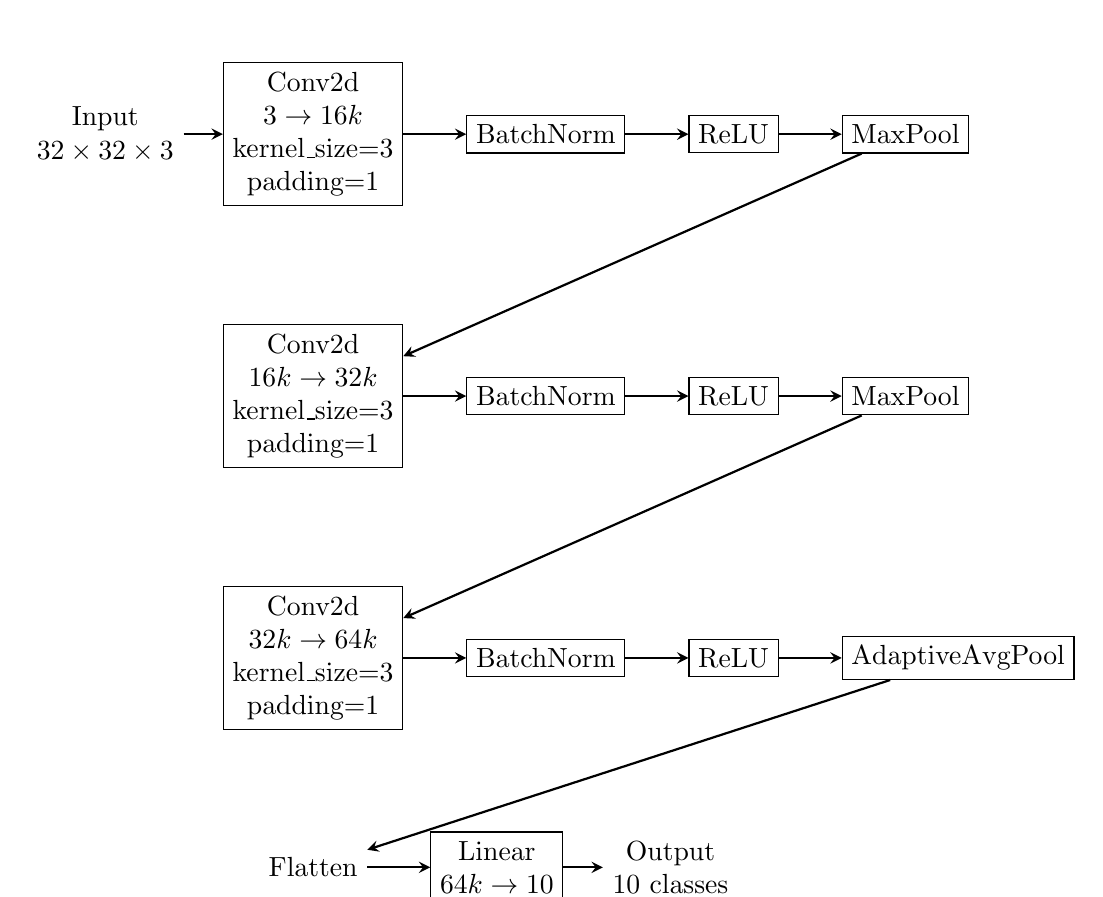
\begin{tikzpicture}[
    node distance=0.8cm,
    conv/.style={draw=black, align=center},
    norm/.style={ draw=black, align=center},
    act/.style={ draw=black, align=center},
    pool/.style={ draw=black, align=center},
    linear/.style={ draw=black, align=center},
    arrow/.style={->, thick, >=stealth},
]
    % Block 1
    \node[conv] (conv1) {Conv2d\\$3 \to 16k$\\kernel\_size=3\\padding=1};
    \node[norm, right=of conv1] (bn1) {BatchNorm};
    \node[act, right=of bn1] (relu1) {ReLU};
    \node[pool, right=of relu1] (pool1) {MaxPool};
    
    % Block 2
    \node[conv, below=1.5cm of conv1] (conv2) {Conv2d\\$16k \to 32k$\\kernel\_size=3\\padding=1};
    \node[norm, right=of conv2] (bn2) {BatchNorm};
    \node[act, right=of bn2] (relu2) {ReLU};
    \node[pool, right=of relu2] (pool2) {MaxPool};
    
    % Block 3
    \node[conv, below=1.5cm of conv2] (conv3) {Conv2d\\$32k \to 64k$\\kernel\_size=3\\padding=1};
    \node[norm, right=of conv3] (bn3) {BatchNorm};
    \node[act, right=of bn3] (relu3) {ReLU};
    \node[pool, right=of relu3] (pool3) {AdaptiveAvgPool};
    
    % Final layers
    \node[below=1.5cm of conv3, minimum width=1.2cm] (flat) {Flatten};
    \node[linear, right=of flat] (linear) {Linear\\$64k \to 10$};
    
    % Arrows within blocks
    \draw[arrow] (conv1) -- (bn1);
    \draw[arrow] (bn1) -- (relu1);
    \draw[arrow] (relu1) -- (pool1);
    
    \draw[arrow] (conv2) -- (bn2);
    \draw[arrow] (bn2) -- (relu2);
    \draw[arrow] (relu2) -- (pool2);
    
    \draw[arrow] (conv3) -- (bn3);
    \draw[arrow] (bn3) -- (relu3);
    \draw[arrow] (relu3) -- (pool3);
    
    \draw[arrow] (pool3) -- (flat);
    \draw[arrow] (flat) -- (linear);
    
    % Vertical connections between blocks
    \draw[arrow] (pool1) -- (conv2);
    \draw[arrow] (pool2) -- (conv3);
    
    % Input
    \node[left=0.5cm of conv1, align=center] (input) {Input\\$32 \times 32 \times 3$};
    \draw[arrow] (input) -- (conv1);
    
    % Output
    \node[right=0.5cm of linear, align=center] (output) {Output\\10 classes};
    \draw[arrow] (linear) -- (output);
\end{tikzpicture}
\caption{Architecture of $\text{ScaledCNN}(k)$.}
\label{fig:scaledcnn}
\end{figure}

\subsubsection{Training Configuration}

To isolate model capacity ($k$) as the independent variable, all other hyperparameters are fixed (Table \ref{tab:hyperparams}). This setup adopts the standard protocol for replicating double descent on CIFAR-10 with label noise \cite{nakkiran2019deep}.

\begin{table}[H]
    \centering
    \caption{Training hyperparameters for ScaledCNN(k).}
    \label{tab:hyperparams}
    \begin{tabular}{ll}
        \toprule
        Hyperparameter & Value \\
        \midrule
        Optimizer & Adam \\
        Learning Rate & $1 \times 10^{-4}$ (constant) \\
        Weight Decay & $0.0$ \\
        Epochs & 500 \\
        \bottomrule
    \end{tabular}
\end{table}

This configuration ensures sufficient time for models to fit the noisy training data, which is required for the "second descent."

\subsubsection{Training and evaluation}

Models with widths $k \in \{1, 2, 4, 8, 16, 32, 64\}$ were trained from scratch on the noisy training set. Final performance was evaluated on the clean test set to plot Test Accuracy vs. Model Capacity.

\subsection{Analysis}

\subsubsection{Statistical Significance}

As the t-test is invalid for comparing correlated classifiers on the same test set (which were trained only once) \cite{compare_two_classifiers}, the non-parametric McNemar's Test \cite{demsar2006statistical} is used to determine if the observed differences are statistically significant ($p < 0.05$). I computed the contingency tables and p-values using the MLxtend library \cite{raschkas_2018_mlxtend}.

\subsubsection{Error Analysis}

Confusion matrices ($10\times10$) are generated for the SVM baseline, the critically-parameterized $\text{ScaledCNN}(k=4)$, and the over-parameterized $\text{ScaledCNN}(k=64)$. These will be analyzed qualitatively to identify changes in inter-class confusion.
\section{Results and Analysis}

\subsection{Classical Baseline Performance}

The SVM + FV baseline achieves a test accuracy of 53.64\% (\autoref{tab:svm_performance}). The confusion matrix (\autoref{fig:svm_confusion}) shows significant errors on certain inter-classes trucks/automobiles and cats/dogs, which suggests the FV features are insufficient for separating visually similar categories.

\begin{table}[H]
    \centering
    \caption{Test-set performance of the SVM + FV baseline.}
    \label{tab:svm_performance}
    \begin{tabular}{lccc}
        \toprule
        Model & Accuracy (\%) & Macro F1 & Weighted F1 \\
        \midrule
        SVM + FV & 53.64 & 0.53 & 0.53 \\
        \bottomrule
    \end{tabular}
\end{table}

\begin{figure}[H]
    \centering
    \includegraphics[width=0.9\textwidth]{figures/SVM__test__confusion_matrix.pdf}
    \caption{Normalized confusion matrix for the SVM + FV baseline on the CIFAR-10 test set.}
    \label{fig:svm_confusion}
\end{figure}

\subsection{Epoch-Wise and Model-Wise Double Descent}

The $\text{ScaledCNN}(k)$ models exhibit both epoch-wise and model-wise double descent.

Epoch-wise double descent appears in wider models ($k \ge 8$, \autoref{fig:scaledcnn_error_curves}). For $k=16$, validation error initially decreases, spikes to $\approx 0.70$ as the model interpolates the noisy training set (train error $\to 0$ near epoch 100), and subsequently recovers to $\approx 0.29$ as the optimizer locates a better-generalizing solution \cite{nakkiran2019deep}.

Model-wise double descent is confirmed by test set performance (\autoref{tab:scaledcnn_test_performance} and \autoref{fig:capacity_curve}). Test accuracy drops from 69.28\% ($k=1$) to a trough of 67.84\% at the interpolation threshold ($k=4$). Beyond this "critically-parameterized" point, accuracy recovers, climbing to a peak of 76.55\% at $k=64$ in the "second descent."

\begin{table}[H]
    \centering
    \caption{Test-set performance of $\text{ScaledCNN}(k)$ on CIFAR-10.}
    \label{tab:scaledcnn_test_performance}
    \begin{tabular}{cccc}
        \toprule
        Width $k$ & Trainable Params & Accuracy (\%) & Macro F1 \\
        \midrule
        1  & $2.4\times 10^{4}$  & 69.28 & 0.69 \\
        2  & $9.5\times 10^{4}$  & 67.87 & 0.68 \\
        4  & $3.7\times 10^{5}$  & 67.84 & 0.67 \\
        8  & $1.5\times 10^{6}$  & 68.43 & 0.66 \\
        16 & $5.9\times 10^{6}$  & 71.02 & 0.71 \\
        32 & $2.4\times 10^{7}$  & 74.29 & 0.74 \\
        64 & $9.4\times 10^{7}$  & 76.55 & 0.77 \\
        \bottomrule
    \end{tabular}
\end{table}

\begin{figure}[H]
    \centering
    \includegraphics[width=0.7\textwidth]{figures/scaledcnn_capacity_vs_performance.pdf}
    \caption{Test accuracy and macro F1 vs. trainable parameters (log scale) for $\text{ScaledCNN}(k)$.}
    \label{fig:capacity_curve}
\end{figure}

\begin{figure}[H]
    \centering
    \includegraphics[width=0.45\textwidth]{figures/scaledcnn_k4_error_curve.pdf}
    \includegraphics[width=0.45\textwidth]{figures/scaledcnn_k16_error_curve.pdf}
    \caption{Epoch-wise train/validation error for $k=4$ (left) and $k=16$ (right). The $k=16$ model shows a clear "dip and recovery" after interpolating the noisy training data.}
    \label{fig:scaledcnn_error_curves}
\end{figure}

\subsection{Statistical and Error Analysis (RQ3)}

\subsubsection{Statistical Significance}

McNemar's test \cite{demsar2006statistical} confirms that the over-parameterized $\text{ScaledCNN}(k=64)$ outperforms the SVM baseline ($p \approx 0$, \autoref{tab:mcnemar_results}).

The test also verifies that the initial accuracy drop from $k=1$ to $k=2$ is significant ($p = 0.0037$), while the difference between $k=2$ and $k=4$ is not ($p = 0.967$), statistically identifying the trough. The recovery in the over-parameterized regime is robust: improvements from $k=8 \to 16$, $k=16 \to 32$, and $k=32 \to 64$ are all significant ($p < 0.001$).

\begin{table}[H]
    \centering
    \caption{McNemar's test results for key model comparisons on the 10,000-sample test set.}
    \label{tab:mcnemar_results}
    \begin{tabular}{llcc}
        \toprule
        Model A & Model B & p-value & Significant \\
        \midrule
        SVM & $\text{ScaledCNN}(k=1)$ & $6.56 \times 10^{-167}$ & Yes \\
        SVM & $\text{ScaledCNN}(k=64)$ & $2.66 \times 10^{-314}$ & Yes \\
        $\text{ScaledCNN}(k=1)$ & $\text{ScaledCNN}(k=2)$ & $3.69 \times 10^{-3}$ & Yes \\
        $\text{ScaledCNN}(k=2)$ & $\text{ScaledCNN}(k=4)$ & $0.967$ & No \\
        $\text{ScaledCNN}(k=4)$ & $\text{ScaledCNN}(k=8)$ & $0.206$ & No \\
        $\text{ScaledCNN}(k=8)$ & $\text{ScaledCNN}(k=16)$ & $1.24 \times 10^{-7}$ & Yes \\
        $\text{ScaledCNN}(k=16)$ & $\text{ScaledCNN}(k=32)$ & $2.34 \times 10^{-12}$ & Yes \\
        $\text{ScaledCNN}(k=32)$ & $\text{ScaledCNN}(k=64)$ & $7.92 \times 10^{-10}$ & Yes \\
        \bottomrule
    \end{tabular}
\end{table}

\subsubsection{Qualitative Error Analysis}

Comparison of confusion matrices (\autoref{fig:svm_confusion}, \autoref{fig:scaledcnn_confusions}) confirms that over-parameterization yields superior inter-class discrimination. The SVM baseline confuses `cat' $\to$ `dog' 19.1\% of the time and still mistakes `bird' for `airplane' 10.3\%. The critically-parameterized $\text{ScaledCNN}(k=4)$ inherits the same weaknesses, misclassifying `bird' $\to$ `airplane' 18.5\% of the time despite modest gains elsewhere.

The over-parameterized $\text{ScaledCNN}(k=64)$ resolves these ambiguities. It reduces `bird' $\to$ `airplane' confusion to 6.2\% and lowers `cat' $\to$ `dog' to 10.6\%, supporting the hypothesis that the implicit regularization of the "second descent" produces more discriminative features.

\begin{figure}[H]
    \centering
    \includegraphics[width=0.45\textwidth]{figures/scaledcnn_k4_test_confusion_matrix.pdf}
    \includegraphics[width=0.45\textwidth]{figures/scaledcnn_k64_test_confusion_matrix.pdf}
    \caption{Normalized confusion matrices for the "peak error" model $\text{ScaledCNN}(k=4)$ (left) and the "second descent" model $\text{ScaledCNN}(k=64)$ (right).}
    \label{fig:scaledcnn_confusions}
\end{figure}

\section{Limitations}

This study relies on the CIFAR-10 dataset and a synthetic uniform label noise model. To ensure the observed event is not an artifact of the low-resolution data or synthetic randomization, future work should validate these findings on other datasets like ImageNet \cite{krizhevsky2012imagenet} and naturally occurring label noise distributions. Specifically, to confirm the scaling laws proposed by Nakkiran et al. \cite{nakkiran2019deep}.

Furthermore, this experiment only tested a plain CNN. Because model biases affect generalization \cite{belkin2019reconciling}, I would have to repeat this scaling study on other architecture (e.g., ResNets, Transformers) to see if model size behaves differently as more depth or attention is added, as hinted by recent large-scale results \cite{zhang2017understanding}.
\section{Conclusion}

This project investigated generalization across the full capacity spectrum, showing that the best over-parameterized CNN, $\text{ScaledCNN}(k=64)$ (76.55\% acc.), decisively outperforms the classical SVM + Fisher Vector baseline (53.64\% acc.).

The $\text{ScaledCNN}(k)$ family exhibits the full model-wise double descent curve: accuracy falls to the interpolation threshold at $k=4$ before climbing again in the over-parameterized regime, where implicit regularization yields qualitatively better error patterns (e.g., markedly fewer `bird'$\to$`airplane' confusions).

Together, these findings reconcile classical and modern generalization theory and show that, when properly regularized, scaling can deliver both higher accuracy and cleaner decision boundaries.


\clearpage
\bibliographystyle{unsrtnat}
\bibliography{bibliography}

\end{document}